\chapter{अपना भोजन पैदा करना}\label{ch:g6:producing-our-food}

तुम्हारे नाश्ते की मेज़ पर रखी कोई भी चीज़ जंगल में यूँ ही नहीं मिली थी।
रोटी का गेहूँ चुनकर सुधारा और उगाया गया था; \omterm{def:g2:animals-grow-up:born}{दूध} उन्हीं के लिए पाले गए
झुंडों से आया; और दही उसी \omterm{def:g2:animals-grow-up:born}{दूध} से, \omterm{def:g1:the-five-senses:sense}{आँखों} से न दिखने वाले अरबों जीवित
मज़दूरों ने \emph{बनाया} था। मनुष्य सजीवों को सँभालकर अपना पेट भरते हैं
--- उन्हें उगाकर, पालकर, और उनमें से कुछ सबसे नन्हों को काम पर लगाकर।
यह अध्याय उसी भोजन-कार्यशाला का चक्कर लगाता है।

\section{उगाना और पालना}

\begin{definition}[फ़सल और पशुधन]\label{def:g6:producing-our-food:farming}
मानव भोजन-उत्पादन पदार्थ-चक्र की दो मंज़िलों पर सजीवों को सँभालता है:
\begin{itemize}
  \item \emph{फ़सल उगाना}\index{फ़सल}: \omterm{def:g5:food-webs:roles}{उत्पादकों} को सँभालना --- गेहूँ,
        आलू, सब्ज़ियाँ, \omterm{prop:g3:flowers-fruits-seeds:transform}{फल} --- उनके \omterm{def:g6:plants-are-producers:matter}{कार्बनिक पदार्थ} के लिए
        (\cref{prop:g6:plants-are-producers:produce});
  \item \emph{पशुपालन}\index{पशुपालन}: \omterm{def:g5:food-webs:roles}{उपभोक्ताओं} को सँभालना ---
        मवेशी, भेड़ें, सूअर, मुर्ग़ियाँ --- उनके
        पदार्थ के निर्माण के लिए
        (\cref{def:g6:matter-from-food:production}): \omterm{def:g2:animals-grow-up:born}{दूध}, माँस, \omterm{def:g2:animals-grow-up:born}{अंडे},
        ऊन।
\end{itemize}
किसान वही \omterm{def:g6:exploring-our-environment:conditions}{परिस्थितियाँ} सँभालते हैं जिनसे यह पुस्तक बार-बार मिलती है:
फ़सलों के लिए \omterm{def:g6:decomposers-and-soil:soil}{मिट्टी} के खनिज (\cref{rem:g4:what-plants-need:soil}), और
\omterm{def:g1:animals-around-us:animal}{जंतुओं} के लिए चारा --- यानी \cref{pb:g6:matter-from-food:1} का पूरा
बहीखाता, जान-बूझकर चलाया हुआ।
\end{definition}

\begin{example}[गेहूँ का खेत होता क्या है]\label{ex:g6:producing-our-food:wheat}
गेहूँ का खेत एक सँभाला हुआ \omterm{def:g6:exploring-our-environment:components}{पर्यावरण} है
(\cref{prop:g5:people-and-nature:managed}), जो एक ही \omterm{def:g5:food-webs:roles}{उत्पादक} के हिसाब
से सधा है: उसकी \omterm{def:g1:plants-around-us:parts}{जड़ों} के लिए \omterm{def:g6:decomposers-and-soil:soil}{मिट्टी} भरी और ढीली की हुई, बुआई
\cref{prop:g2:from-seed-to-plant:needs} की गरमाहट के हिसाब से, और
खरपतवार --- यानी \cref{ch:g6:how-plants-spread} के प्रतिद्वंद्वी
उपनिवेशी --- बाहर रखे हुए। \omterm{def:g6:producing-our-food:farming}{फ़सल} \omterm{def:g1:plants-around-us:plant}{पौधे} का बीज-भंडार है: अनाज, यानी
दस लाख कभी न बोए जाने वाले गेहूँ के \omterm{def:g1:plants-around-us:plant}{पौधों} के बँधे हुए भोजन, जो
बेकरियों की ओर मोड़ दिए गए।
\end{example}

\begin{remark}[हर भोजन जीवन-चक्र की कोई अवस्था है]\label{rem:g6:producing-our-food:stage}
किसी भी भोजन को \omterm{def:g1:living-or-not:living}{जीवविज्ञान} की नज़र से पढ़ो और वह किसी जीव का अंग या
अवस्था निकलता है: अनाज और सेम बीज-भंडार हैं; आलू \omterm{ex:g4:plants-without-seeds:bulbtuber}{कंद}; सेब वे \omterm{prop:g3:flowers-fruits-seeds:transform}{फल} जो खाए
जाने के लिए ही बने हैं (\cref{exo:g6:how-plants-spread:12}); \omterm{def:g2:animals-grow-up:born}{दूध}
\omterm{prop:g3:sorting-living-things:groups}{स्तनधारी} माँ की देखभाल है (\cref{def:g2:animals-grow-up:born}); और \omterm{def:g2:animals-grow-up:born}{अंडा}
एक बँधा हुआ पालनाघर। भोजन-उत्पादन \omterm{def:g2:born-grow-die:cycle}{जीवन चक्रों} को इस तरह सँभालने की कला
है कि उनका सामान हमारी मेज़ों तक पहुँचे।
\end{remark}

\section{अदृश्य कार्यबल: सूक्ष्मजीवों का बनाया भोजन}

\begin{definition}[किण्वन]\label{def:g6:producing-our-food:fermentation}
कुछ भोजन \omterm{def:g1:the-five-senses:sense}{आँखों} से न दिखने वाले सजीवों --- यानी
\emph{सूक्ष्मजीवों}\index{सूक्ष्मजीव (भोजन में)} --- को किसी कच्चे माल
पर काम पर लगाकर बनाए जाते हैं। उनका खाना उस माल को बदल देता है: इसी
बदलाव को \emph{किण्वन}\index{किण्वन} कहते हैं, और मनुष्य इसे हज़ारों
साल से चला रहे हैं, यानी तब से जब किसी को यह पता तक नहीं था कि ये
मज़दूर होते भी हैं।
\end{definition}

\begin{example}[रोटी फूलती है]\label{ex:g6:producing-our-food:bread}
रोटी का कच्चा गूँधा हुआ आटा आटे और पानी का होता है --- और साथ में
\emph{खमीर}\index{खमीर}, यानी एककोशिकीय \omterm{def:g6:decomposers-and-soil:decomposers}{कवक}
(\cref{rem:g5:first-look-at-cells:onecelled} में ऐसे ही जीवन से भेंट
हुई थी)। \omterm{ex:g6:producing-our-food:bread}{खमीर} आटे की शक्कर पर पलता है और एक गैस छोड़ता है; और उस गैस के
बुलबुले लचीले आटे में फँसकर उसे फुला देते हैं --- नानबाई इसी को फूलना
कहता है। फिर ओवन की गरमी मज़दूरों की पाली ख़त्म कर देती है और उनका काम
जमा देती है: भीतर के छेद \omterm{ex:g6:producing-our-food:bread}{खमीर} के ही दस्तख़त हैं।
\end{example}

\begin{omfigure}
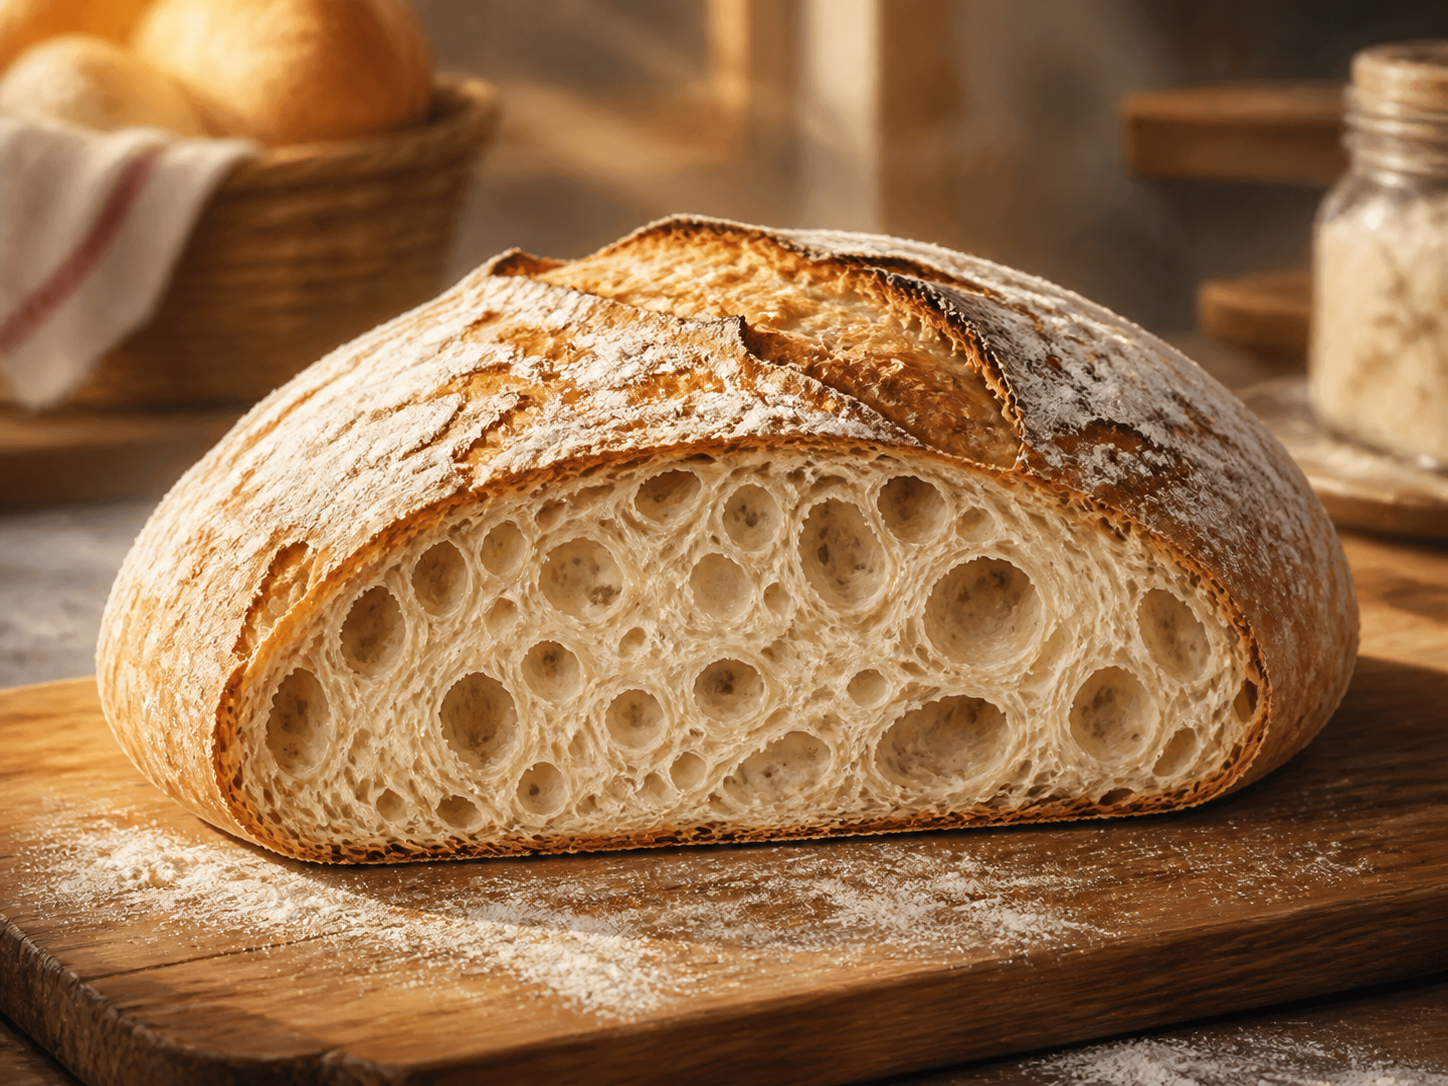
\includegraphics[width=0.58\linewidth]{images/book1/ai/g6-food-bread.png}

{\small कार्यबल के दस्तख़त, वहीं पके हुए: भीतर का हर छेद वह बुलबुला है
जो \omterm{ex:g6:producing-our-food:bread}{खमीर} ने फुलाया था।}
\end{omfigure}

\begin{example}[दूध दही और पनीर बनता है]\label{ex:g6:producing-our-food:yogurt}
सही \omterm{def:g6:producing-our-food:fermentation}{सूक्ष्मजीवों} का जामन डाला हुआ गरम \omterm{def:g2:animals-grow-up:born}{दूध} रात भर में जमकर दही बन जाता
है: मज़दूर \omterm{def:g2:animals-grow-up:born}{दूध} की शक्कर पर पलते हैं और एक अम्ल छोड़ते हैं, और वही अम्ल
\omterm{def:g2:animals-grow-up:born}{दूध} को जमा देता है --- वह ताज़ा खटास \emph{ही} वह अम्ल है। पनीर भी इसी
तरह शुरू होता है, पर आगे जाता है: दही को दबाया, नमक लगाया और महीनों
पकाया जाता है, और उस पकने के दौरान सूक्ष्मजीव काम करते रहते हैं ---
किसी पनीर के छेद, ऊपरी परत और तेज़ महक उनकी लंबी पाली का ही रोज़नामचा
हैं।
\end{example}

\begin{remark}[मददगार और नुक़सानदेह सूक्ष्मजीव]\label{rem:g6:producing-our-food:goodbad}
\cref{def:g1:healthy-habits:germs} के \omterm{def:g1:healthy-habits:germs}{रोगाणुओं} ने \omterm{def:g6:producing-our-food:fermentation}{सूक्ष्मजीवों} से
सावधानी सिखाई थी; यह अध्याय उसका दूसरा आधा हिस्सा जोड़ता है:
\emph{चुने हुए} सूक्ष्मजीव, \emph{क़ाबू में रखी} \omterm{def:g6:exploring-our-environment:conditions}{परिस्थितियों} में काम
करते हुए, हमारे सबसे पुराने कर्मचारियों में हैं --- रोटी में, दही में,
पनीर में, और सिरके के पीपे में। कारीगरी हमेशा वही है: चुने हुए मज़दूरों
का स्वागत करो, और ऐसी \omterm{def:g6:exploring-our-environment:conditions}{परिस्थितियाँ} रखो जो उन्हें भाएँ, बिगाड़ने वालों
को नहीं। नमक लगाना, ठंडा रखना, सुखाना और पकाना, सब अनचाहे \omterm{def:g6:producing-our-food:fermentation}{सूक्ष्मजीवों}
को \omterm{def:g6:exploring-our-environment:conditions}{परिस्थितियाँ} देने से इनकार करने के ही तरीक़े हैं
(\cref{prop:g6:decomposers-and-soil:speed} किसी हैम पर ठीक वैसे ही काम
करता है जैसे पत्तों के ढेर पर)।
\end{remark}

\section{खेत से मेज़ तक, ईमानदारी से}

\begin{proposition}[मेज़ पर चढ़े दाम]\label{prop:g6:producing-our-food:costs}
हर थाली सँभाली हुई ज़मीन और सँभाले हुए सजीवों की उपज है, और उन्हीं का
गणित अपने साथ लाती है:
\begin{itemize}
  \item \omterm{def:g1:plants-around-us:plant}{पौधों} के भोजन \omterm{def:g6:exploring-our-environment:conditions}{प्रकाश} से एक ही मंज़िल दूर पहुँचते हैं; \omterm{def:g1:animals-around-us:animal}{जंतुओं} के
        भोजन पहले किसी \omterm{def:g5:food-webs:roles}{उपभोक्ता} से होकर जाते हैं और
        \cref{prop:g6:matter-from-food:losses} का चुंगी-कर चुकाते हैं
        (\cref{exo:g6:matter-from-food:12});
  \item टिकाऊ उत्पादन को \cref{prop:g5:people-and-nature:lasting} के
        तीनों नियम निभाने ही होते हैं --- \omterm{def:g6:decomposers-and-soil:soil}{मिट्टी} को खिलाओ, मददगारों को
        बचाओ, और भरने से ज़्यादा तेज़ी से मत लो;
  \item और बरबादी यह सब बेकार कर देती है: फेंका गया भोजन अपनी ज़मीन,
        पानी और मेहनत किसी के लिए भी ख़र्च नहीं करता।
\end{itemize}
\end{proposition}
\admitted

\begin{method}[किसी भोजन की कहानी पढ़ना]\label{met:g6:producing-our-food:read}
रसोई के किसी भी भोजन के लिए:
\begin{enumerate}
  \item उस जीव का नाम बताओ और यह भी कि वह उसका कौन-सा अंग या अवस्था है
        (\cref{rem:g6:producing-our-food:stage});
  \item उसे चक्र पर रखो: \omterm{def:g5:food-webs:roles}{उत्पादक} का पदार्थ, \omterm{def:g5:food-webs:roles}{उपभोक्ता} का उत्पाद, या
        \omterm{def:g6:producing-our-food:fermentation}{सूक्ष्मजीवों} का बनाया हुआ?
  \item अगर \omterm{def:g6:producing-our-food:fermentation}{सूक्ष्मजीवों} का बनाया है, तो कच्चे माल का नाम बताओ और यह
        भी कि मज़दूरों ने क्या बदला;
  \item उसका पीछा उसकी \omterm{def:g1:plants-around-us:parts}{पत्ती} तक करो
        (\cref{met:g6:plants-are-producers:trace}) --- रास्ता आज भी
        हमेशा \omterm{def:g6:exploring-our-environment:conditions}{प्रकाश} पर ही ख़त्म होता है।
\end{enumerate}
\end{method}

\begin{example}[नाश्ते पर यह विधि]\label{ex:g6:producing-our-food:breakfast}
दही, इस विधि से: (1) \omterm{def:g2:animals-grow-up:born}{दूध} --- गाय की माँ-देखभाल का उत्पाद --- बदला
हुआ; (2) \omterm{def:g5:food-webs:roles}{उपभोक्ता} का उत्पाद, \omterm{def:g6:producing-our-food:fermentation}{सूक्ष्मजीवों} से पूरा किया हुआ; (3) कच्चा
माल \omterm{def:g2:animals-grow-up:born}{दूध}, और मज़दूरों ने उसे खट्टा करके जमा दिया; (4) \omterm{def:g2:animals-grow-up:born}{दूध} गाय से, गाय
घास से, और घास \omterm{def:g6:exploring-our-environment:conditions}{प्रकाश} से। तीन जीव और अरबों का एक कार्यबल, एक छोटी-सी
कटोरी में।
\end{example}

\section{अभ्यास}

\begin{exercise}[$\star$]\label{exo:g6:producing-our-food:1}
\omterm{def:g6:producing-our-food:farming}{फ़सल उगाने} और \omterm{def:g6:producing-our-food:farming}{पशुपालन} की परिभाषा दो, और हर एक के साथ पदार्थ-चक्र की वह
मंज़िल भी बताओ जिसे वह सँभालता है।
\end{exercise}

\begin{exercise}[$\star$]\label{exo:g6:producing-our-food:2}
हर भोजन के लिए जीव और उसका अंग या अवस्था बताओ: अनाज, आलू, सेब, \omterm{def:g2:animals-grow-up:born}{दूध},
\omterm{def:g2:animals-grow-up:born}{अंडा}।
\end{exercise}

\begin{exercise}[$\star$]\label{exo:g6:producing-our-food:3}
\omterm{def:g6:producing-our-food:fermentation}{किण्वन} क्या है? दो किण्वित भोजन और उनके कच्चे माल बताओ।
\end{exercise}

\begin{exercise}[$\star$]\label{exo:g6:producing-our-food:4}
बताओ कि रोटी क्यों फूलती है: मज़दूर, उसका भोजन, वह क्या छोड़ता है, और
ओवन क्या करता है।
\end{exercise}

\begin{exercise}[$\star$]\label{exo:g6:producing-our-food:5}
\omterm{def:g2:animals-grow-up:born}{दूध} को दही में क्या जमा देता है, और वह खटास कहाँ से आती है?
\end{exercise}

\begin{exercise}[$\star$]\label{exo:g6:producing-our-food:6}
\cref{rem:g6:producing-our-food:goodbad} से अनचाहे \omterm{def:g6:producing-our-food:fermentation}{सूक्ष्मजीवों} को
\omterm{def:g6:exploring-our-environment:conditions}{परिस्थितियाँ} देने से इनकार करने के तीन तरीक़े बताओ।
\end{exercise}

\begin{exercise}[$\star\star$]\label{exo:g6:producing-our-food:7}
गेहूँ का खेत \cref{prop:g4:what-plants-need:needs} की हर ज़रूरत
जान-बूझकर सँभालता है। हर ज़रूरत को
\cref{ex:g6:producing-our-food:wheat} में बताए किसान के काम से मिलाओ।
\end{exercise}

\begin{exercise}[$\star\star$]\label{exo:g6:producing-our-food:8}
पनीर पर \cref{met:g6:producing-our-food:read} चरण दर चरण चलाओ।
\end{exercise}

\begin{exercise}[$\star\star$]\label{exo:g6:producing-our-food:9}
फ़्रिज भोजन को क्यों बचाए रखता है --- और वही ठंड खाद के ढेर को धीमा
क्यों कर देती है? एक ही सिद्धांत, दो रसोइयाँ: उसका नाम बताओ।
\end{exercise}

\begin{exercise}[$\star\star$]\label{exo:g6:producing-our-food:10}
\cref{def:g1:healthy-habits:germs} को इस अध्याय से मिलाओ: सूक्ष्मजीव
एक साथ हाथ धुलवाने वाले दुश्मन और दही का कार्यबल, दोनों कैसे हो सकते
हैं?
\end{exercise}

\begin{exercise}[$\star\star$]\label{exo:g6:producing-our-food:11}
\cref{prop:g6:producing-our-food:costs} की मदद से समझाओ कि फेंका गया
हैम का सैंडविच उतने ही वज़न की फेंकी गई रोटी से ज़्यादा बरबादी क्यों
है।
\end{exercise}

\begin{exercise}[$\star\star\star$]\label{exo:g6:producing-our-food:12}
हज़ारों साल तक नानबाई और शराब बनाने वाले \omterm{def:g6:producing-our-food:fermentation}{किण्वन} चलाते रहे, जबकि उन्हें
पता ही नहीं था कि सूक्ष्मजीव होते भी हैं। असल में वे किस चीज़ को
सँभालते थे, \cref{prop:g6:exploring-our-environment:decide} की भाषा
में --- और उनकी तरकीबें फिर भी काम क्यों करती थीं?
\end{exercise}

\section{समस्या: कक्षा की बेकरी}

\begin{problem}[{सप्ताहांत समस्या --- रोटी का एक बैच, बीज से टुकड़े तक
पीछा किया हुआ}]\label{pb:g6:producing-our-food:1}
स्कूल के मेले के लिए कक्षा शुरू से रोटी बनाती है --- और जुलाई में गेहूँ
के खेत की सैर से लेकर नवंबर की रोटियों तक अपनी \omterm{def:g1:living-or-not:living}{जीवविज्ञान} की कॉपी खुली
रखती है।

\medskip\noindent\textbf{भाग I --- खेत (जुलाई)।}
\begin{enumerate}
  \item किसान पका हुआ गेहूँ दिखाता है: ``यह \omterm{def:g6:producing-our-food:farming}{फ़सल} \omterm{def:g1:plants-around-us:plant}{पौधे} के बँधे हुए भोजन
        हैं।'' \cref{def:g2:from-seed-to-plant:seed} की मदद से इस
        वाक्य को खोलो --- हर दाना क्या है, और वह किसके लिए बाँधा गया
        था?
  \item अनाज का \omterm{def:g6:plants-are-producers:matter}{कार्बनिक पदार्थ} किसकी \omterm{def:g1:plants-around-us:parts}{पत्तियों} में, और किन सामग्रियों
        से बना था?
  \item किसान अगले पतझड़ \omterm{def:g6:producing-our-food:farming}{फ़सल} का सिर्फ़ एक हिस्सा बोता है और बाक़ी बेच
        देता है। गेहूँ के दाने की दोनों नियतियाँ जीवन-चक्र की भाषा में
        बताओ।
  \item \omterm{def:g6:producing-our-food:farming}{फ़सल} के बाद खेत की \omterm{def:g6:decomposers-and-soil:soil}{मिट्टी} को खाद मिलती है। यह कौन-सा लौटाने
        वाला नियम है, और यह \omterm{def:g1:plants-around-us:plant}{पौधे} की पाँचों ज़रूरतों में से किसकी सेवा
        करता है?
\end{enumerate}

\medskip\noindent\textbf{भाग II --- बेकरी (नवंबर)।}
\begin{enumerate}[resume]
  \item कक्षा आटा, पानी, नमक और \omterm{ex:g6:producing-our-food:bread}{खमीर} मिलाती है, और गूँधा हुआ आटा किसी
        गरम कोने में रख देती है। गरम क्यों? \omterm{ex:g6:producing-our-food:bread}{खमीर} के लिए वैसे ही उत्तर
        दो जैसे किसी भी जीवित मज़दूर के लिए
        (\cref{prop:g6:decomposers-and-soil:speed} में यह ढर्रा है)।
  \item घंटे भर बाद आटा दुगुना हो चुका है। इस फूलने को समझाओ: \omterm{ex:g6:producing-our-food:bread}{खमीर} ने
        किस पर पोषण लिया, उसने क्या छोड़ा, और उसे फँसाया किसने?
  \item एक टोली का आटा, जो हवा वाली ठंडी खिड़की के पास भूल गया था,
        मुश्किल से फूलता है। जाँच करो --- और बताओ कि दोनों टोलियों ने
        अनजाने में कौन-सी न्यायी-जाँच वाली तुलना चला दी।
  \item ओवन में रोटियाँ फूलना बंद कर देती हैं और जम जाती हैं। गरमी ने
        कार्यबल का क्या किया, और भीतर उसके दस्तख़त के रूप में क्या बचा
        रह जाता है?
\end{enumerate}

\medskip\noindent\textbf{भाग III --- हिसाब।}
\begin{enumerate}[resume]
  \item तैयार टुकड़े का पीछा कड़ी दर कड़ी \omterm{def:g6:exploring-our-environment:conditions}{प्रकाश} तक करो।
  \item मेले में मक्खन और हैम के सैंडविच भी बिकते हैं। टुकड़े, मक्खन
        और हैम को उन मंज़िलों के हिसाब से क्रम में लगाओ जिनसे उनका
        पदार्थ होकर गुज़रा, और बताओ कि किसने
        \cref{prop:g6:matter-from-food:losses} का सबसे बड़ा चुंगी-कर
        चुकाया।
  \item बिना बिका आटा कूड़ेदान में नहीं, खाद में जाता है। उसके \omterm{def:g6:plants-are-producers:matter}{कार्बनिक
        पदार्थ} का चक्र में एक मोड़ और पीछा करो --- उसे कौन लेता है, और
        किस ओर?
  \item कॉपी एक वाक्य से बंद करो, जिसमें ये हों: \omterm{def:g5:food-webs:roles}{उत्पादक}, \omterm{def:g5:food-webs:roles}{उपभोक्ता}
        (अगर कोई हो), \omterm{def:g6:producing-our-food:fermentation}{सूक्ष्मजीवों} का कार्यबल, और \omterm{def:g6:exploring-our-environment:conditions}{प्रकाश}।
\end{enumerate}
\end{problem}
